% This file was created with tikzplotlib v0.10.1.
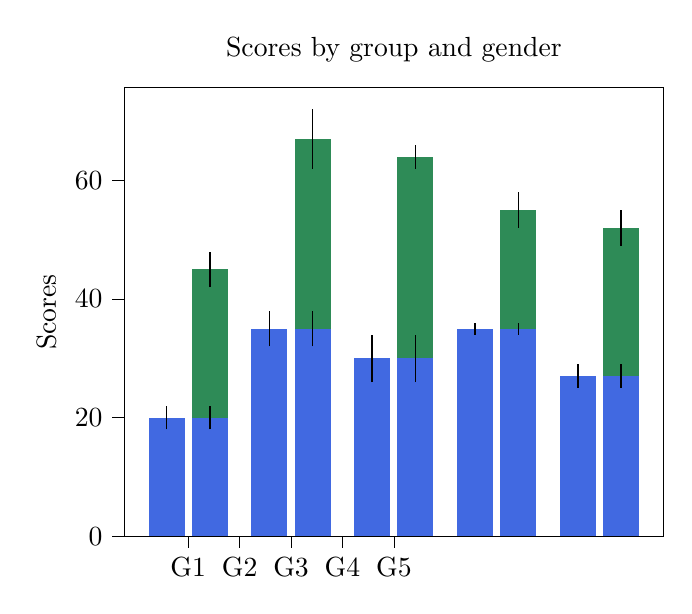
\begin{tikzpicture}

\definecolor{darkgray176}{RGB}{176,176,176}
\definecolor{royalblue}{RGB}{65,105,225}
\definecolor{seagreen}{RGB}{46,139,87}

\begin{axis}[
tick align=outside,
tick pos=left,
title={Scores by group and gender},
x grid style={darkgray176},
xmin=-0.4135, xmax=4.8335,
xtick style={color=black},
xtick={0.21,0.71,1.21,1.71,2.21},
xticklabels={G1,G2,G3,G4,G5},
y grid style={darkgray176},
ylabel={Scores},
ymin=0, ymax=75.6,
ytick style={color=black}
]
\draw[draw=none,fill=royalblue] (axis cs:-0.175,0) rectangle (axis cs:0.175,20);
\draw[draw=none,fill=royalblue] (axis cs:0.825,0) rectangle (axis cs:1.175,35);
\draw[draw=none,fill=royalblue] (axis cs:1.825,0) rectangle (axis cs:2.175,30);
\draw[draw=none,fill=royalblue] (axis cs:2.825,0) rectangle (axis cs:3.175,35);
\draw[draw=none,fill=royalblue] (axis cs:3.825,0) rectangle (axis cs:4.175,27);
\draw[draw=none,fill=royalblue] (axis cs:0.245,0) rectangle (axis cs:0.595,20);
\draw[draw=none,fill=royalblue] (axis cs:1.245,0) rectangle (axis cs:1.595,35);
\draw[draw=none,fill=royalblue] (axis cs:2.245,0) rectangle (axis cs:2.595,30);
\draw[draw=none,fill=royalblue] (axis cs:3.245,0) rectangle (axis cs:3.595,35);
\draw[draw=none,fill=royalblue] (axis cs:4.245,0) rectangle (axis cs:4.595,27);
\draw[draw=none,fill=seagreen] (axis cs:0.245,20) rectangle (axis cs:0.595,45);
\draw[draw=none,fill=seagreen] (axis cs:1.245,35) rectangle (axis cs:1.595,67);
\draw[draw=none,fill=seagreen] (axis cs:2.245,30) rectangle (axis cs:2.595,64);
\draw[draw=none,fill=seagreen] (axis cs:3.245,35) rectangle (axis cs:3.595,55);
\draw[draw=none,fill=seagreen] (axis cs:4.245,27) rectangle (axis cs:4.595,52);
\path [draw=black, semithick]
(axis cs:0,18)
--(axis cs:0,22);

\path [draw=black, semithick]
(axis cs:1,32)
--(axis cs:1,38);

\path [draw=black, semithick]
(axis cs:2,26)
--(axis cs:2,34);

\path [draw=black, semithick]
(axis cs:3,34)
--(axis cs:3,36);

\path [draw=black, semithick]
(axis cs:4,25)
--(axis cs:4,29);

\path [draw=black, semithick]
(axis cs:0.42,18)
--(axis cs:0.42,22);

\path [draw=black, semithick]
(axis cs:1.42,32)
--(axis cs:1.42,38);

\path [draw=black, semithick]
(axis cs:2.42,26)
--(axis cs:2.42,34);

\path [draw=black, semithick]
(axis cs:3.42,34)
--(axis cs:3.42,36);

\path [draw=black, semithick]
(axis cs:4.42,25)
--(axis cs:4.42,29);

\path [draw=black, semithick]
(axis cs:0.42,42)
--(axis cs:0.42,48);

\path [draw=black, semithick]
(axis cs:1.42,62)
--(axis cs:1.42,72);

\path [draw=black, semithick]
(axis cs:2.42,62)
--(axis cs:2.42,66);

\path [draw=black, semithick]
(axis cs:3.42,52)
--(axis cs:3.42,58);

\path [draw=black, semithick]
(axis cs:4.42,49)
--(axis cs:4.42,55);

\end{axis}

\end{tikzpicture}
